\documentclass[tikz,border=4pt]{standalone}
\usepackage{amsmath,amssymb}
\usetikzlibrary{positioning,arrows.meta,fit,backgrounds,calc}

% Color palette conforming to specification:
% Energy solid #D55E00, Information dashed #0072B2
\definecolor{cEnergy}{HTML}{D55E00}
\definecolor{cInfo}{HTML}{0072B2}
\definecolor{cHub}{HTML}{F0F4F8}
\definecolor{cBox}{HTML}{FFFFFF}

\tikzset{
  % Component box
  box/.style={
    draw=black!75,
    rounded corners=2pt,
    align=center,
    font=\scriptsize,
    minimum height=8.5mm,
    inner sep=3pt,
    fill=cBox,
    line width=0.6pt
  },
  % Central controller hub
  hub/.style={
    draw=black!85,
    rounded corners=3pt,
    align=center,
    font=\scriptsize,
    minimum height=15mm,
    inner sep=5pt,
    fill=cHub,
    line width=1.2pt
  },
  % Energy flow (solid #D55E00)
  energy/.style={
    -{Stealth[length=1.8mm, width=1.3mm]},
    cEnergy,
    line width=1.15pt
  },
  energyBi/.style={
    {Stealth[length=1.8mm, width=1.3mm]}-{Stealth[length=1.8mm, width=1.3mm]},
    cEnergy,
    line width=1.15pt
  },
  % Information flow (dashed #0072B2)
  info/.style={
    -{Stealth[length=1.8mm, width=1.3mm]},
    cInfo,
    line width=1.0pt,
    densely dashed
  },
  infoBi/.style={
    {Stealth[length=1.8mm, width=1.3mm]}-{Stealth[length=1.8mm, width=1.3mm]},
    cInfo,
    line width=1.0pt,
    densely dashed
  },
  % Bus conductor line
  bus/.style={
    cEnergy,
    line width=1.8pt
  },
  % Group boundary
  group/.style={
    draw=black!40,
    dashed,
    rounded corners=3pt,
    inner sep=4pt
  }
}

\begin{document}
\begin{tikzpicture}[>=Stealth]

  % ==========================================
  % TOP ROW: Grid, Generation, Storage, EV
  % ==========================================
  % External Grid & Smart Meter
  \node[box, text width=2.1cm, fill=gray!10] (grid) at (-6.1, 2.6) {\textbf{Grid}\\\textbf{Connection}\\\vspace{1pt}\scriptsize External Utility};
  \node[box, text width=1.9cm] (meter) at (-3.4, 2.6) {\textbf{Smart Meter}\\\vspace{1pt}\scriptsize Bi-directional};

  % Rooftop PV
  \node[box, text width=2.2cm] (pv) at (-0.8, 2.6) {\textbf{Rooftop PV}\\\textbf{Array}\\\vspace{1pt}\scriptsize Solar Generation};

  % Home Battery (ESS)
  \node[box, text width=2.4cm] (ess) at (1.8, 2.6) {\textbf{Home Battery}\\\textbf{(ESS)}\\\vspace{1pt}\scriptsize Energy Storage};

  % Electric Vehicle with Charger
  \node[box, text width=3.0cm] (ev) at (5.0, 2.6) {\textbf{Electric Vehicle (EV)}\\\textbf{with EV Charger}\\\vspace{1pt}\scriptsize V2H / V2G Capable};

  % ==========================================
  % MIDDLE ROW: Thermostatic Loads, Central Controller, Legend
  % ==========================================
  % Thermostatically Controllable Loads (Left)
  \node[box, text width=2.3cm] (hvac) at (-5.4, 0.7) {\textbf{HVAC Unit}\\\vspace{1pt}\scriptsize Heating / Cooling};
  \node[box, text width=2.3cm] (wh) at (-5.4, -0.7) {\textbf{Electric}\\\textbf{Water Heater}\\\vspace{1pt}\scriptsize Thermal Buffer};

  % Central HEMS Controller (RL Agent)
  \node[hub, text width=4.6cm] (hems) at (0.0, 0.0) {
    \textbf{\normalsize Central HEMS Controller}\\[2pt]
    \textbf{\footnotesize Reinforcement-Learning Agent}\\[3pt]
    \tiny State Sensing $\cdot$ Action Dispatch\\[1pt]
    \tiny Policy Optimization (DQN / PPO / SAC)
  };

  % Legend Box (Right)
  \node[draw=black!50, rounded corners=3pt, fill=white, inner sep=4pt, text width=2.6cm, line width=0.6pt] (legend) at (5.2, 0.0) {
    \centering\textbf{\scriptsize Flow Legend}\\[3pt]
    \raggedright
    \begin{tikzpicture}[baseline=-0.5ex]
      \draw[energy, line width=1.1pt] (0,0) -- (0.5,0);
    \end{tikzpicture}\hspace{3pt}{\tiny Energy Flow}\\[2pt]
    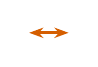
\begin{tikzpicture}[baseline=-0.5ex]
      \draw[energyBi, line width=1.1pt] (0,0) -- (0.5,0);
    \end{tikzpicture}\hspace{3pt}{\tiny Bi-dir. Energy}\\[2pt]
    \begin{tikzpicture}[baseline=-0.5ex]
      \draw[info, line width=0.9pt] (0,0) -- (0.5,0);
    \end{tikzpicture}\hspace{3pt}{\tiny Info / Status}\\[2pt]
    
\begin{tikzpicture}[baseline=-0.5ex]
      \draw[infoBi, line width=0.9pt] (0,0) -- (0.5,0);
    \end{tikzpicture}\hspace{3pt}{\tiny Control / State}
  };

  % ==========================================
  % BOTTOM ROW: Deferrable Loads, Fixed Loads
  % ==========================================
  % Deferrable Loads (Shiftable)
  \node[box, text width=1.55cm] (wm) at (-5.0, -2.5) {\textbf{Washing}\\\textbf{Machine}};
  \node[box, text width=1.2cm] (dryer) at (-3.4, -2.5) {\textbf{Dryer}};
  \node[box, text width=1.65cm] (dw) at (-1.7, -2.5) {\textbf{Dishwasher}};

  % Fixed Loads (Non-shiftable)
  \node[box, text width=1.75cm] (fridge) at (1.5, -2.5) {\textbf{Refrigerator}};
  \node[box, text width=1.2cm] (light) at (3.3, -2.5) {\textbf{Lighting}};
  \node[box, text width=1.4cm] (vac) at (5.0, -2.5) {\textbf{Vacuum}\\\textbf{Cleaner}};

  % Side Labels for Load Groups (clean, completely avoids all lines)
  \node[align=center, font=\scriptsize\bfseries, text=black!80] (def_label) at (-6.8, -2.5) {Deferrable\\Loads\\\tiny (Shiftable)};
  \node[align=center, font=\scriptsize\bfseries, text=black!80] (fix_label) at (6.7, -2.5) {Fixed\\Loads\\\tiny (Baseline)};

  % ==========================================
  % GROUP BOXES (Backgrounds)
  % ==========================================
  \begin{scope}[on background layer]
    % TCL group
    \node[group, fit=(hvac)(wh), label={[anchor=south, yshift=2pt]above:\scriptsize\bfseries Controllable Thermal Loads}] (tcl_group) {};

    % Deferrable group
    \node[group, fit=(def_label)(wm)(dryer)(dw)] (def_group) {};

    % Fixed group
    \node[group, fit=(fridge)(light)(vac)(fix_label)] (fix_group) {};
  \end{scope}

  % ==========================================
  % HOME AC POWER BUS (Perimeter Ring)
  % ==========================================
  \coordinate (busTL) at (-7.5, 3.8);
  \coordinate (busTR) at (7.5, 3.8);
  \coordinate (busBR) at (7.5, -3.8);
  \coordinate (busBL) at (-7.5, -3.8);

  % Draw bus lines
  \draw[bus] (busTL) -- (busTR) -- (busBR) -- (busBL) -- cycle;
  \node[above=1pt, font=\scriptsize\bfseries, text=cEnergy] at (0, 3.8) {Home AC Power Bus};
  \node[below=1pt, font=\scriptsize\bfseries, text=cEnergy] at (0, -3.8) {Home AC Power Bus};

  % ==========================================
  % ENERGY FLOWS (Solid Orange)
  % ==========================================
  % Grid <-> Smart Meter
  \draw[energyBi] (grid.east) -- (meter.west);

  % Smart Meter <-> Bus (Bi-directional exchange with grid)
  \draw[energyBi] (meter.north) -- (meter.north |- busTL);

  % PV -> Bus (Unidirectional solar generation)
  \draw[energy] (pv.north) -- (pv.north |- busTL);

  % ESS <-> Bus (Charge / Discharge)
  \draw[energyBi] (ess.north) -- (ess.north |- busTL);

  % EV with Charger <-> Bus (Charge / V2H Discharge)
  \draw[energyBi] (ev.north) -- (ev.north |- busTL);

  % Bus -> HVAC & Water Heater (from Left Bus Trunk)
  \draw[energy] (busTL |- hvac.west) -- (hvac.west);
  \draw[energy] (busBL |- wh.west) -- (wh.west);

  % Bus -> Deferrable Loads (from Bottom Bus)
  \draw[energy] (wm.south |- busBL) -- (wm.south);
  \draw[energy] (dryer.south |- busBL) -- (dryer.south);
  \draw[energy] (dw.south |- busBL) -- (dw.south);

  % Bus -> Fixed Loads (from Bottom Bus)
  \draw[energy] (fridge.south |- busBL) -- (fridge.south);
  \draw[energy] (light.south |- busBL) -- (light.south);
  \draw[energy] (vac.south |- busBL) -- (vac.south);

  % ==========================================
  % INFORMATION FLOWS (Dashed Blue)
  % ==========================================
  % HEMS <-> Smart Meter (Tariffs & Net Exchange)
  \draw[infoBi] (hems.140) -- (meter.south);

  % PV -> HEMS (Solar generation telemetry)
  \draw[info] (pv.south) -- (hems.105);

  % HEMS <-> ESS (SoC monitoring & Charge/Discharge commands)
  \draw[infoBi] (hems.75) -- (ess.south);

  % HEMS <-> EV (Battery status, trip deadline & Charging control)
  % Routed cleanly above legend to ev.205
  \draw[infoBi] (hems.50) -- (ev.205);

  % HEMS <-> HVAC & Water Heater (Temperatures & Setpoint control)
  \draw[infoBi] (hvac.east) -- (hems.165);
  \draw[infoBi] (wh.east) -- (hems.195);

  % HEMS <-> Deferrable Loads (Run requests & scheduled activation)
  \draw[infoBi] (hems.225) -- (wm.north);
  \draw[infoBi] (hems.242) -- (dryer.north);
  \draw[infoBi] (hems.258) -- (dw.north);

  % Fixed Loads -> HEMS (Power consumption monitoring / baseline profile)
  \draw[info] (fridge.north) -- (hems.282);
  \draw[info] (light.north) -- (hems.298);
  \draw[info] (vac.north) -- (hems.315);

\end{tikzpicture}
\end{document}
